% !TEX root = ../../I4PRJ, Grp3 - Dokumentation.tex
\section{Applikationslaget}
I dette afsnit beskrives designet af applikationslaget. Applikationslaget er det lag af software i det samlede distribuerede system, som installeres eller afvikles hos brugeren. Applikationslaget er designet til at være platformuafhængigt, jf. systemets arkitektur. Derved er lagets model- og præsentationslag designet til at være portabelt, hvorimod view-laget er platformspecifikt. På figur~\ref{fig:application_layer} ses det overordnede lagdiagram for applikationslagets design.

\begin{figure}
	\centering
	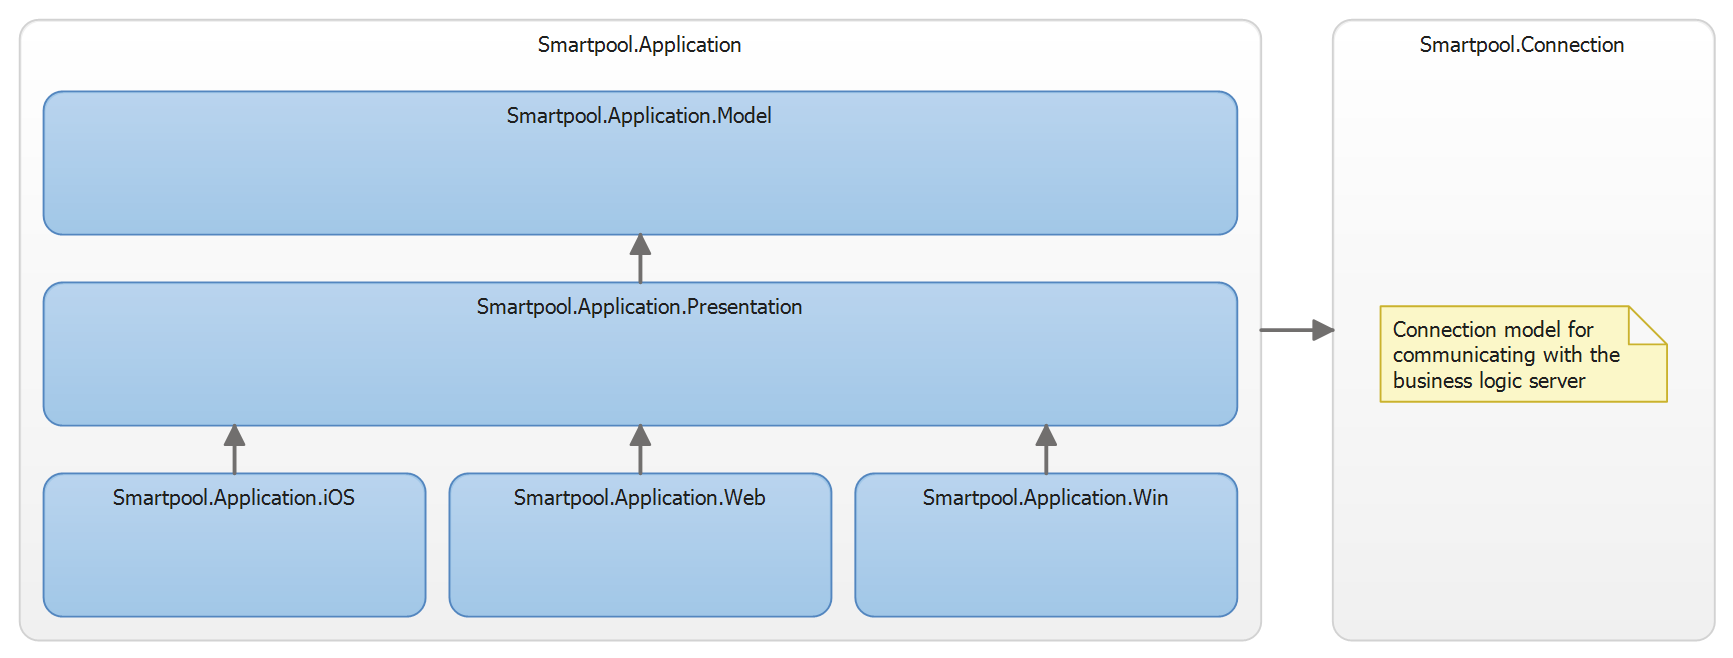
\includegraphics[width=1.0\linewidth]{figs/design/application_layer}
	\caption{Lagdiagram applikationslagets softwarepakker}
	\label{fig:application_layer}
\end{figure}

Af diagrammet fremgår det, at applikationslaget er opdelt i flere lag som følge af model-view-presenter arkitekturen, beskrevet i afsnittet arkitektur. En del af applikationslagets model findes i en separat pakke under navnet Smartpool.Connection. Denne pakke indeholder model-klasser til kommunikation mellem klient-applikationerne og Smartpools businesss-logic server.

Som følge af multi-lag arkitekturen kunne applikationslaget samt de platform-specifikke view-implementeringer designes, uafhængigt af hinanden, så længe interfaces blev specificeret undervejs i processen. Sammenkobling og protokolspecificering mellem de forskellige lag i applikationen er et resultat af interface specificeringen. Et eksempel på dette er rækken af view/presenter interfaces beskrevet i underafsnittet om design af applikationens præsentationslag.

Den overordnede ide omkring designet af model-view-presenter er adskillelse af lagene. View kalder presenter, som kan hente data fra model. Opstarts- og et interaktionsscenarie eksemplificeres på sekvensdiagrammet på figur~\ref{fig:application_sd}.

\begin{figure}
	\centering
	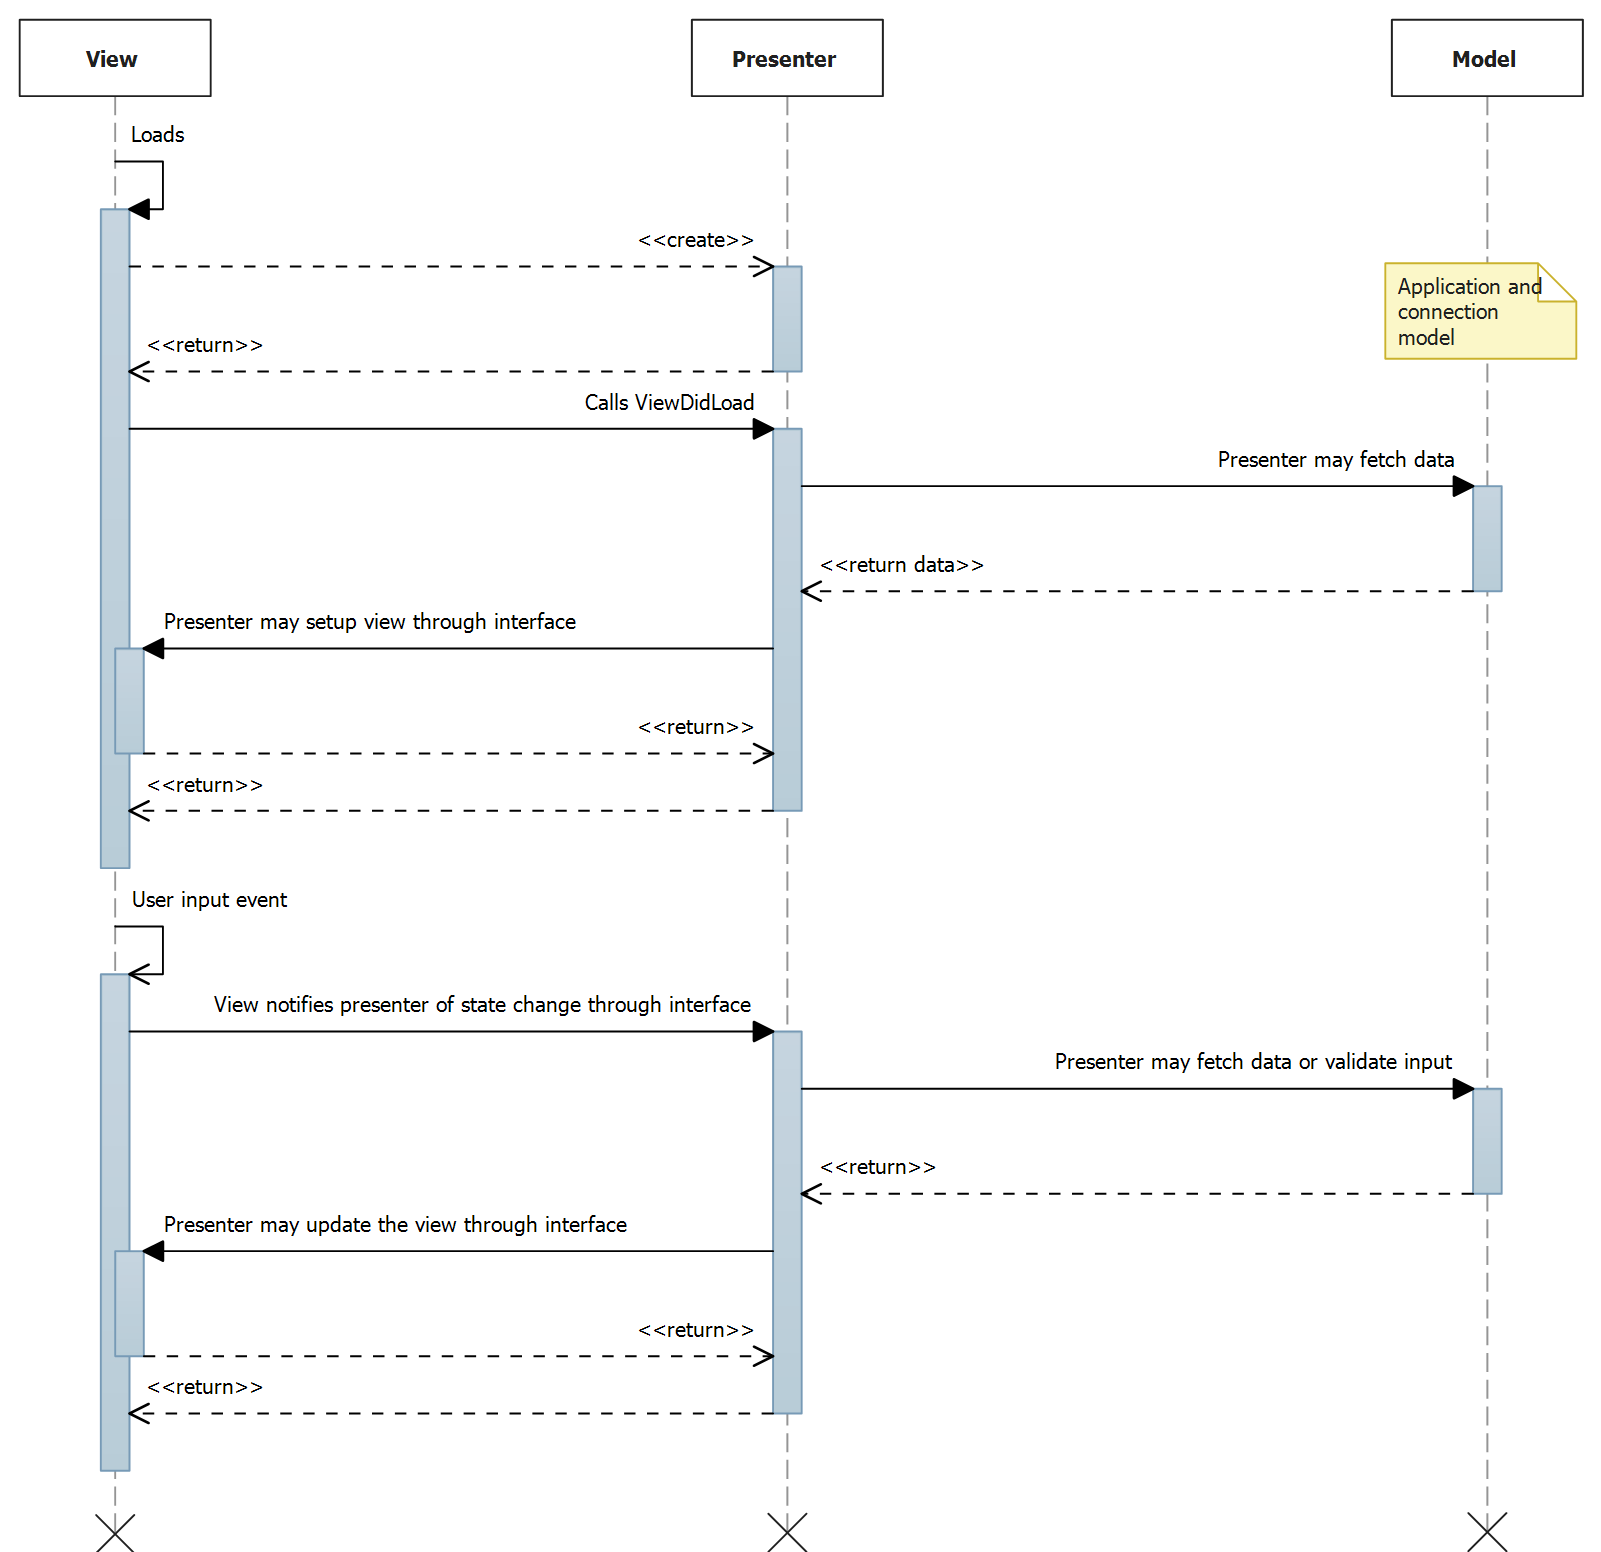
\includegraphics[width=1.0\linewidth]{figs/design/application_sd}
	\caption{Sekvensdiagram for det generelle interaktionsmønster i applikationslaget}
	\label{fig:application_sd}
\end{figure}

\subsection{Applikationens modellag}
I dette afsnit beskrives designet af softwarepakken Smartpool.Application.Model. Modellaget består af de klasser der håndterer beregninger og verificering af data lokalt, inden data sendes fra applikationslaget til serveren. I modellaget findes også klasser der gemmer klient-applikationens tilstand i runtime.

Modellaget har til formål at adskille den førnævnte logik fra præsentations- og view-laget, for at overholde applikationslagets overordnede model-view-presenter arkitektur, samt at genbruge rutiner der anvendes af flere forskellige presenters. Klassediagrammet for applikationens modellag kan ses på figur~\ref{fig:application_model_cd}

\begin{figure}
	\centering
	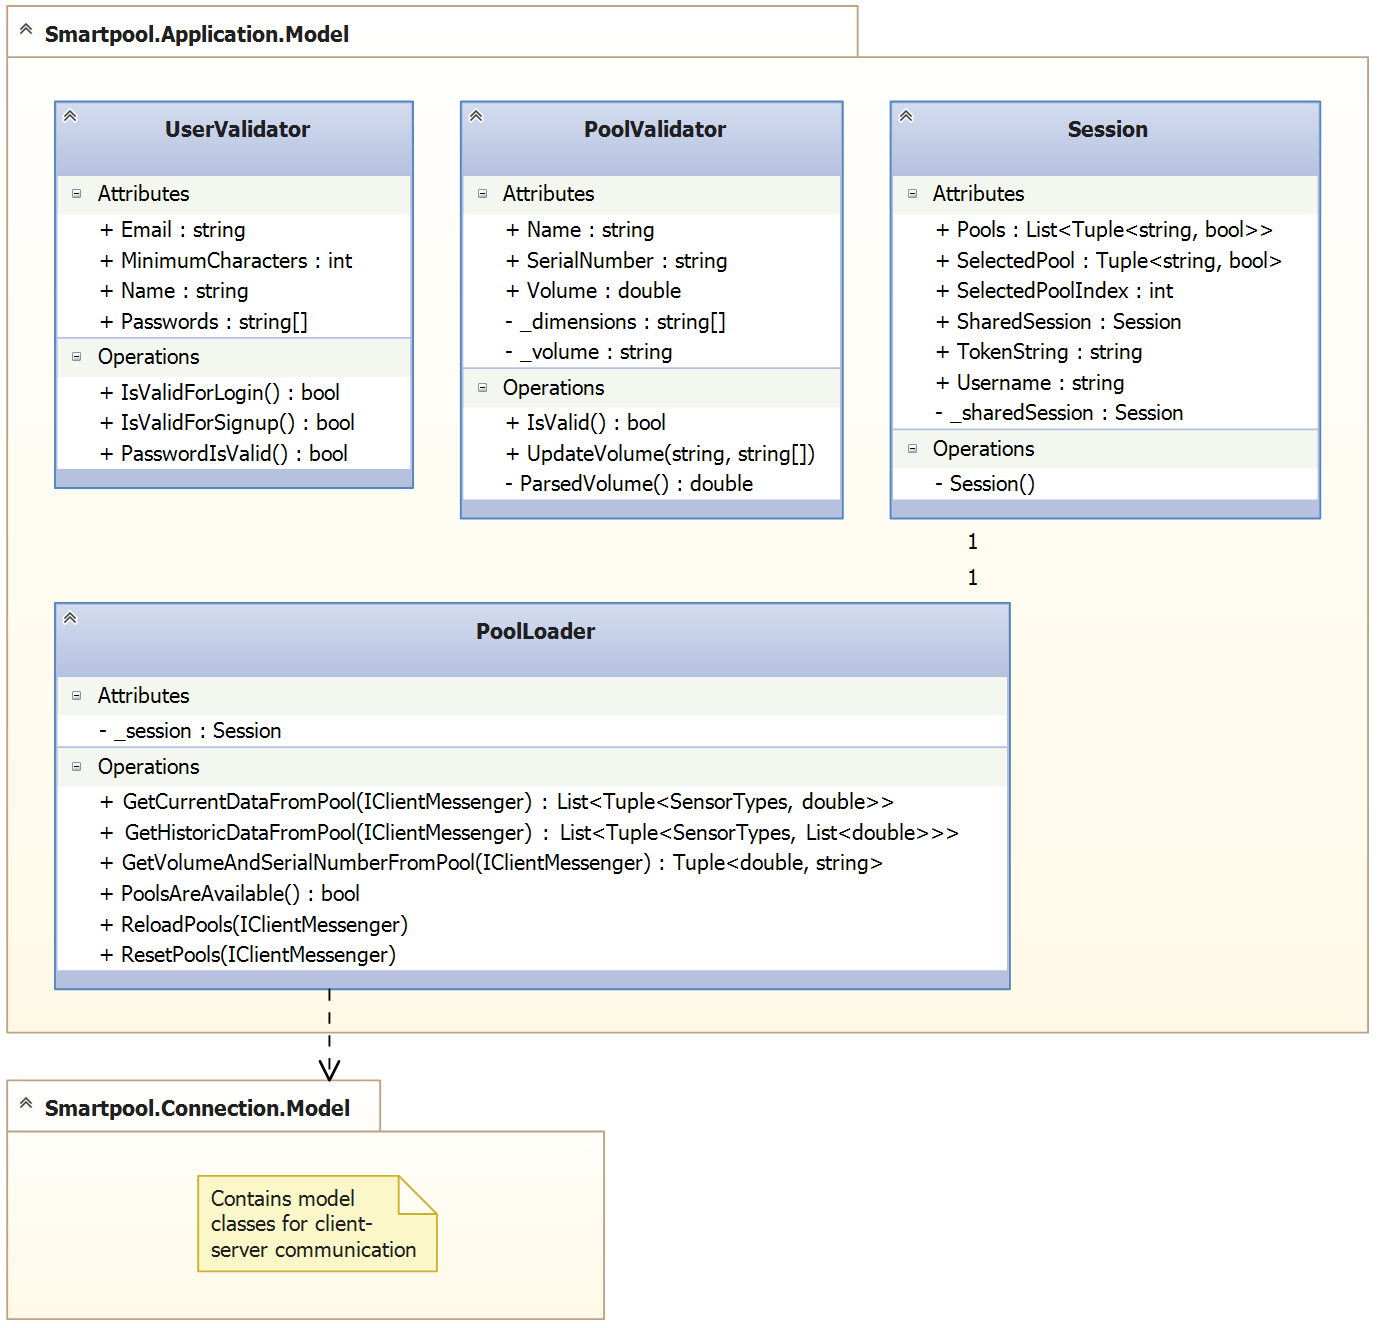
\includegraphics[width=1.0\linewidth]{figs/design/application_model_cd}
	\caption{Applikationens modellag}
	\label{fig:application_model_cd}
\end{figure}

Af diagrammet fremgår det at denne softwarepakke består af fire klasser. Det bemærkes desuden modellen har en afhængighed til Smartpool.Connection.Model, som indeholder den yderligere forbindelsesmodel, der deles af både applikationslaget og connection-server laget. I de efterfølgende afsnit beskrives de enkelte klassers design.

\subsubsection{Session}

Session er en klasse der skal gemme applikationens tilstand i runtime. Session-klassen blev designet ud fra client-server aspektet af systemets arkitektur, således at sessionsoplysninger fra serveren kunne lagres midlertidigt i applikationslaget. Session-klassen er designet som en singleton, således at applikationens tilstand kan persistere mellem overgange til forskellige views og presenters.

I Session-klassen gemmes information modtaget fra serveren (Username og TokenString) efter en forbindelse er blevet oprettet. Derudover gemmes information om hvilken pool brugeren har valgt at interagere med. En beskrivelse af Session-klassens medlemmer fremgår af tabel~\ref{tab:table_design_session}

\begin{table}
	\centering
	\begin{tabular}{| l | p{0.7\linewidth} |}
		\toprule
		\textbf{Klassemedlem}	& \textbf{Beskrivelse} \\
		\midrule
		+ Pools		& En liste med pools. En pool repræsenteres med navn og notifikationsstatus.		\\\hline
		+ SelectedPool			& En property som returnerer den pool som brugeren sidst har valgt at undersøge.	\\\hline
		+ SelectedPoolIndex				& En integer der tilsvarer den valgte pools index i listen af pools.				\\\hline
		+ SharedSession				& En property der returnere den statiske instans af Session-klassen, eller konstruere den hvis den ikke allerede findes, som følge af Singleton princippet. \\\hline
		+ TokenString					& En string indeholdende et token der bruges til kontakt med serveren. \\\hline
		+ Username						& En string indeholdende det brugernavn som brugeren af applikationen er logget ind med. \\\hline
		- sharedSession					& Backing variablen til den statiske Singleton Session. \\\hline
		- Session()							& Session-klassens constructor. Den er gjort privat for at sikre Singleton-metoden. \\
		\bottomrule
		\end{tabular}
	\caption{Beskrivelse af Session-klassens medlemmer}
	\label{tab:table_design_session}	
\end{table}

\subsubsection{PoolLoader}
PoolLoader er en klasse der har til ansvar at indkapsle den logik der omfatter indlæsning og overføring af pool-data fra client-server forbindelsen, til Session-klassen i applikationslaget. 

PoolLoader-klassen indeholder en række metoder der gør det nemmere for klasser i præsentationslaget at udføre førnævnte opgaver, således at præsentationsklasserne der indlæser pool-oplysninger kan fralægge sig dele af dette ansvar, og fokusere på præsentationslogik.

\begin{table}
	\centering
	\begin{tabular}{| l | p{0.5\linewidth} |}
		\toprule
		\textbf{Klassemedlem}	& \textbf{Beskrivelse} \\
		\midrule
		- session					& En reference til Singleton-instansen i Session-klassen, som skal bruges til lagring af information om brugerens session. \\\hline
		+ GetCurrentDataFromPool(...)	& En metode der returnere øjebliksdata fra den aktive pool i Session-instansen.	\\\hline
		+ GetHistoricDataFromPool(...) 	& En metode der returnere historisk data fra den aktive pool i Session-instansen. \\\hline
		+ GetVolumeAndSerialNumberFromPool(...)	& En metode der returnere volumen og serienummer på aktive pool i Session-instansen. \\\hline
		+ PoolsAreAvailable() 					& En metode der returnere en boolean værdi, som angiver hvorvidt Pools-listen i klassens Session-instans indeholder pools. \\\hline
		+ ReloadPools(...)						& Metoder til at indlæse eller genindlæse listen af pools på brugerens konto. \\
		+ ResetPools(...)						&  \\
		\bottomrule
		\end{tabular}
	\caption{Beskrivelse af PoolLoader-klassens medlemmer}
	\label{tab:table_design_poolloader}	
\end{table}

Mange af metoderne i PoolLoader-klassen tager imod en IClientMessenger. Denne klasse anvendes primært som interface til klienten i applikationslaget. Med interfacet kan beskeder sendes til serveren. Det er nødvendigt da PoolLoader-klassen sørger for at sende de forskellige pool-data beskeder til serveren, som kræves for at indhente den fornødne data.

\subsubsection{PoolValidator}
PoolValidator er en klasse der indkapsler valideringslogik for klasser i præsentationslaget, der enten har med oprettelse eller modificering af pools at gøre.

Klassen indeholder de properties som en almindelig pool også indeholder, samt metoder der kan kaldes for at undersøge om klassens properties er sat korrekt, i forhold til det der forventes af en pool i systemet.

\begin{table}
	\centering
	\begin{tabular}{| l | p{0.7\linewidth} |}
		\toprule
		\textbf{Klassemedlem}	& \textbf{Beskrivelse} \\
		\midrule
		+ Name				& Tekststrenge der bør sættes i forbindelse med validering af en ny pool.	\\
		+ SerialNumber			& 	\\\hline
		+ Volume 				& En property der returnere en double-repræsentation af den private volume tekststreng. \\\hline
		- dimensions 			& Private klassemedlemmer der kan indeholde oplysninger om poolens størrelse og volumen. \\
		- volume 				& 	\\\hline
		+ IsValid()					& En metode der returnere en boolean værdi, som angiver hvorvidt klassens state tillader dannelse af en ny pool. \\\hline
		+ UpdateVolume(...)						& En metode der tager imod størrelse og volumen, og opdatere de private klassemedlemmer volume og dimensions. \\\hline
		- ParsedVolume					& En metode der omdanner de to private klassemedlemmer volume og dimensions, til en double værdi. \\
		\bottomrule
		\end{tabular}
	\caption{Beskrivelse af PoolValidator-klassens medlemmer}
	\label{tab:table_design_poolvalidator}	
\end{table}

\subsubsection{UserValidator}
UserValidator er en klasse der håndterer validering af brugeroprettelse og redigering på applikationslaget, inden en forespørgsel af denne type sendes til serveren.

Klassen hjælper med at isolere brugervalideringslogik, fra klasser i præsentationslaget som håndterer brugerredigering, samt at give præsentationslaget mulighed for at sende feedback opdateringer til view-laget. Dette er også med til at aflaste serveren, da en forespørgsel med ufuldendte oplysninger ikke kan sendes til validering på serveren, mens UserValidator-klassen benyttes.

\begin{table}
	\centering
	\begin{tabular}{| l | p{0.7\linewidth} |}
		\toprule
		\textbf{Klassemedlem}	& \textbf{Beskrivelse} \\
		\midrule
		+ Name				& Tekststrenge der bør sættes i forbindelse med validering af en ny bruger.	\\
		+ Email 			& 	\\\hline
		+ MinimumCharacters  				& En integer der angiver det mindst mulige antal af karaktere der kan indgå i brugerens password. MinimumCharacters er const og kan derfor kun læses udefra. MinimumCharacters bruges af PasswordIsValid metoden til at vurdere hvorvidt et password er gyldigt. \\\hline
		+ Passwords  			& En array af tekststrenge der bruges til at gemme de passwords som indtastes af brugeren. Et array af passwords er nødvendigt da to passwords skal sammenlignes for at sikre at brugeren har indtastet passwordet rigtigt gentagende gange.\\\hline
		+ IsValidForLogin() 				& En metode der returnere en boolean værdi, som angiver hvorvidt UserValidator-klassens state tillader login. I denne metode tjekkes medlemsvariablerne Name og Passwords. \\\hline
		+ IsValidForSignup() 			& En metode der returnere en boolean værdi, som angiver hvorvidt UserValidator-klassens state tillader brugeroprettelse. I denne metode tjekkes alle medlemsvariablerne.
 \\\hline
		+ PasswordIsValid()				& En metode der sammenligner de passwords som er gemt i medlemsvariablen Passwords, og returnere en boolean der angiver hvorvidt de er ens. \\
		\bottomrule
		\end{tabular}
	\caption{Beskrivelse af UserValidator-klassens medlemmer}
	\label{tab:table_design_uservalidator}	
\end{table}

\subsection{Applikationens præsentationslag}
I dette afsnit beskrives designet af softwarepakken Smartpool.Application.Presentation. Denne pakke indeholder præsentationslogikken, som indgår i applikationslager, i det distribuerede system.

I præsentationslaget designes en række presenter-interfaces. Disse presenters har til formål at binde model- og view-lag sammen, samt at definere den tilhørende præsentationslogik. Konkrete presenter-klasser er også designet i dette lag. De konkrete klasser implementerer de førnævnte interfaces, samt benytter sig af modellen beskrevet i forrige afsnit. Der defineres også en række view-interfaces. Disse interfaces benyttes og implementeres af view klasser i de platform-specifikke udgaver af Smartpool applikationen. Interfaces er designet undervejs i projektudviklingsforløbet, i takt med at user stories er blevet åbnet og løst.

\subsection{Presenter-interfaces}
Presenter-interfacene definerer en simpel protokol mellem view og presenter. De indeholder metoder som bør kaldes af det tilhørende view, når bestemte events sker i view-laget. Overordnede presenter interfaces er i løbet af projektforløbet blevet identificeret, og segregeret fra de øvrige interfaces.

\begin{figure}
	\centering
	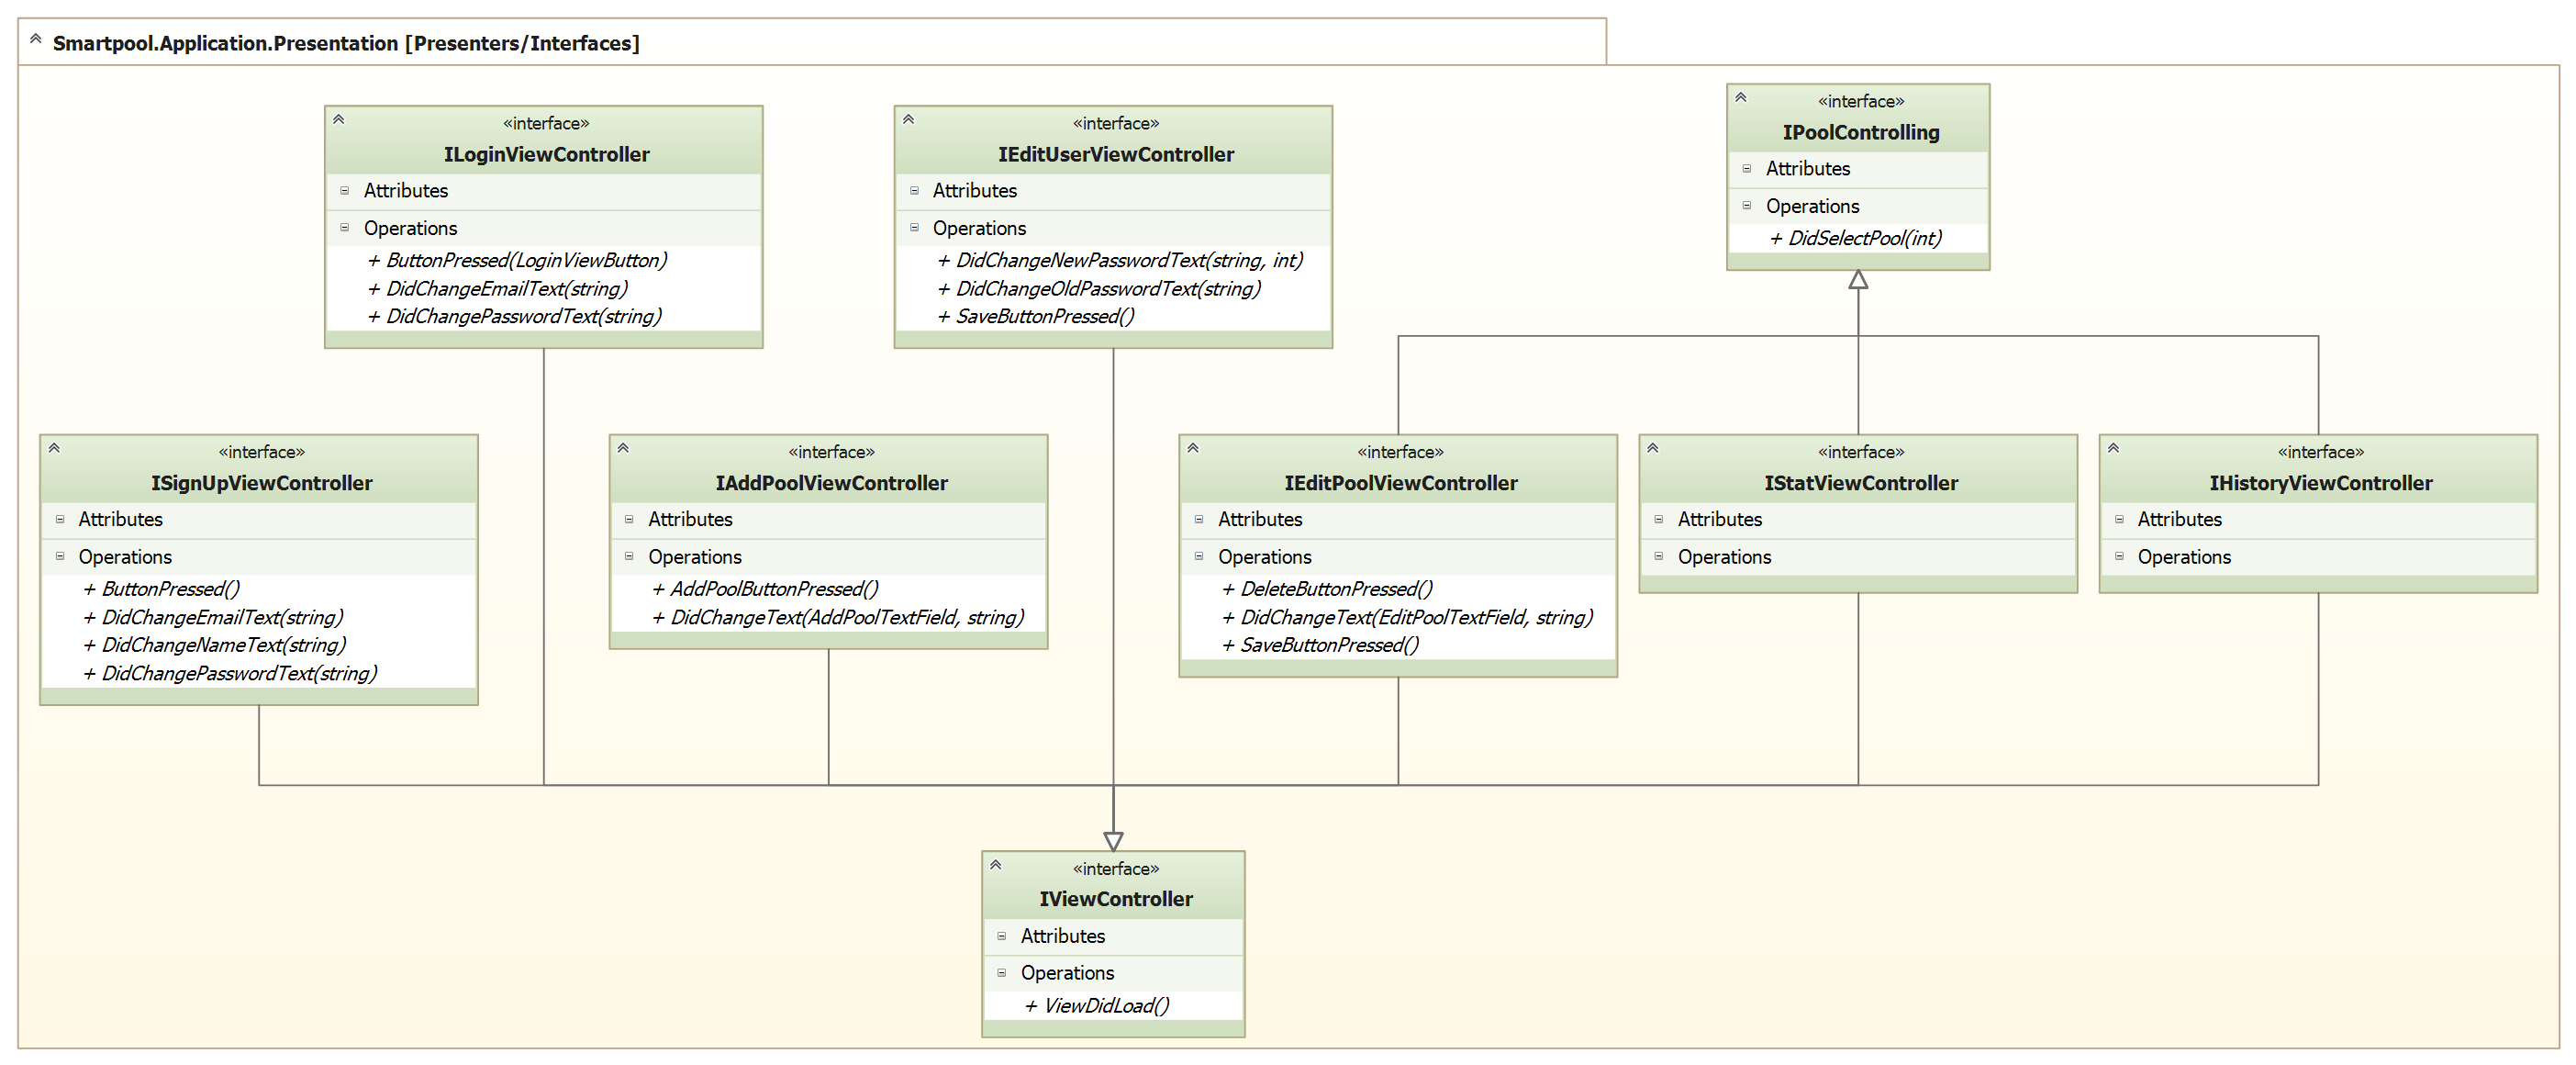
\includegraphics[width=1.0\linewidth]{figs/design/application_presentation_interfaces}
	\caption{Presenter interfaces}
	\label{fig:application_presentation_interfaces}
\end{figure}\todo{skal muligvis på en pdf for sig, så man har en change for at læse det.}

I de efterfølgende afsnit beskrives designet af de forskellige presenter-interfaces.

\subsubsection{IViewController}
IViewController interfacet er det mest generelle presenter-interface, som implementeres af alle de andre presenter-interfaces. Interfacet indeholder en metode, ViewDidLoad, som kaldes af det tilhørende view, efter view´et er loaded i hukommelsen og vises for brugeren.

\begin{figure}
	\centering
	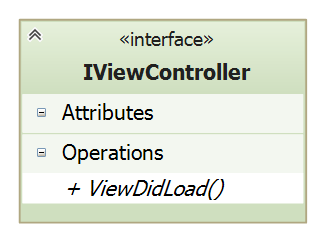
\includegraphics[width=0.3\linewidth]{figs/design/application_iviewcontroller}
	\caption{IViewController}
	\label{fig:application_iviewcontroller}
\end{figure}

\subsubsection{IPoolControlling}
IPoolControlling er et interface der er segregeret fra de interfaces som håndterer visning og styring af pool oplysninger. Interfacet indeholder en metode, DidSelectPool(int), som bør kaldes af det tilhørende view, efter en pool er valgt i view´et, fra en liste eller lignende. Integer parameteren repræsenterer indekset på den valgte pool, i listen af pools (se Session).  
\begin{figure}
	\centering
	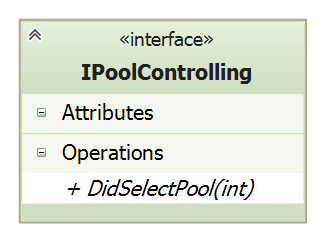
\includegraphics[width=0.3\linewidth]{figs/design/application_ipoolcontrolling}
	\caption{IPoolControlling}
	\label{fig:application_ipoolcontrolling}
\end{figure}

\subsubsection{ISignUpViewController}
Interfacet er designet i forbindelse med user stories, der omhandler, at brugeren skal kunne oprette sig i systemet. Interfacet indeholder metoder, som det tilhørende view kan kalde, når events som tekst-input sker. Dermed kan presenteren, der implementerer interfacet få opdateringer fra viewet, når brugeren indtaster sine oplysninger.

\begin{table}
	\centering
	\begin{tabular}{| l | p{0.65\linewidth} |}
		\toprule
		\textbf{Klassemedlem}	& \textbf{Beskrivelse} \\
		\midrule
		+ ButtonPressed()				& En metode der kaldes af presenterens view, når brugeren fra view'et vælger at færdiggøre brugeroprettelsen.	\\\hline
		+ DidChangeEmailText(...) 			& Metoder der skal kaldes af view?et, når brugeren har indtastet tekst i de pågældende tekstfelter. \\
		+ DidChangeNameText(...)  			& \\\hline
		+ DidChangePasswordText(...) 				& En metode der kaldes af presenterens view, når brugeren indtaster sit ønskede password fra view'et. Passwordet skal indtastes to gange i view?et for at sikre, at det er korrekt indtastet. Metoden indeholder derfor en integer parameter som sættes til enten 0 eller 1, efter hvilken gang passwordet er indtastet. \\
		\bottomrule
		\end{tabular}
	\caption{Beskrivelse af ISignUpViewController-klassens medlemmer}
	\label{tab:table_design_isignupviewcontroller}	
\end{table}

\subsubsection{ILoginViewController}
ILoginViewController interfacet implementeres af den presenter, der håndterer brugerens loginanmodninger. Interfacet indeholder metoder, som view?et kan kalde, når events som tekst-input sker.

\begin{table}
	\centering
	\begin{tabular}{| l | p{0.65\linewidth} |}
		\toprule
		\textbf{Klassemedlem}	& \textbf{Beskrivelse} \\
		\midrule
		+ ButtonPressed()				& En metode der kaldes af presenterens view, når en brugeren trykker på en knap eller et link i view?et. Metoden indeholder en parameter, som er en enumeration over de knapper der kan eksistere i et login view.	\\\hline
		+ DidChangeEmailText(...) 			& Metoder der skal kaldes af view?et, når brugeren har indtastet tekst i de pågældende tekstfelter. \\
		+ DidChangePasswordText(...) 				& \\
		\bottomrule
		\end{tabular}
	\caption{Beskrivelse af ILoginViewController-klassens medlemmer}
	\label{tab:table_design_iloginviewcontroller}	
\end{table}

\subsubsection{IAddPoolViewController}
Dette interface er designet i forbindelse med user stories, der omhandler oprettelse af pools, på en brugers konto. Interfacet indeholder metoder, som view?et kan kalde, når events som tekst-input sker.

\begin{table}
	\centering
	\begin{tabular}{| l | p{0.65\linewidth} |}
		\toprule
		\textbf{Klassemedlem}	& \textbf{Beskrivelse} \\
		\midrule
		+ AddPoolButtonPressed()				& En metode der kaldes af presenterens view, når brugeren ønsker at gennemføre oprettelsen af poolen.	\\\hline
		+ DidChangeText(...) 					& En metode der kaldes af view?et, når brugeren indtaster tekst i et af view?ets tekstfelter. Teksten sendes  sammen med tekstfeltets id. \\
		\bottomrule
		\end{tabular}
	\caption{Beskrivelse af IAddPoolViewController-klassens medlemmer}
	\label{tab:table_design_iaddpoolviewcontroller}	
\end{table}

\subsubsection{IEditUserViewController}
Dette interface er designet i forbindelse med user stories, der omhandler redigering af brugeroplysninger. Interfacet er i første omgang designet ud fra en enkelt user story, der omhandler ændring af brugens password. Interfacet indeholder der metoder, som view?et kan kalde, når brugeren indtaster ønskede password ændringer.

\begin{table}
	\centering
	\begin{tabular}{| l | p{0.6\linewidth} |}
		\toprule
		\textbf{Klassemedlem}	& \textbf{Beskrivelse} \\
		\midrule
		+ DidChangeNewPasswordText(...)				& En metode der kaldes af view?et, når brugeren indtaster sit nye password. Passwordet skal indtastes to gange i view?et for at sikre, at det er korrekt indtastet. Metoden indeholder derfor en integer parameter som sættes til enten 0 eller 1, efter hvilken gang passwordet er indtastet.	\\\hline
		+ DidChangeOldPasswordText(...)				& En metoder der skal kaldes af view?et, når brugeren indtaster sit gamle password. \\\hline
		+ SaveButtonPressed() 					& En metode der kaldes af view?et, når brugeren ønsker at gennemføre sin oprettelse. \\
		\bottomrule
		\end{tabular}
	\caption{Beskrivelse af IEditUserViewController-klassens medlemmer}
	\label{tab:table_design_iedituserviewcontroller}	
\end{table}

\subsubsection{IEditPoolViewController}
IEditPoolViewController interfacet er designet i forbindelse med user stories der omhandler redigering af pools, på en brugers konto.

\begin{table}
	\centering
	\begin{tabular}{| l | p{0.7\linewidth} |}
		\toprule
		\textbf{Klassemedlem}	& \textbf{Beskrivelse} \\
		\midrule
		+ DeleteButtonPressed()				& Metoder der kaldes når brugeren vælger at slette eller gemme ændringer for en given pool.	\\
		+ SaveButtonPressed				& \\\hline
		+ DidChangeText(...) 					& En metode der kaldes af view?et, når brugeren indtaster tekst i et af view?ets tekstfelter. Teksten sendes  sammen med tekstfeltets id. \\
		\bottomrule
		\end{tabular}
	\caption{Beskrivelse af IEditPoolViewController-klassens medlemmer}
	\label{tab:table_design_ieditpoolviewcontroller}	
\end{table}

\subsubsection{IStatViewController og IHistoryViewController}
Disse interfaces er begge en komposition af IViewController og IPoolControlling. Dette virker umiddelbart redundant men skyldes forventet fremtidig funktionalitet, der endnu ikke er en del af de to interfaces. De to interfaces implementeres af presenter-klasser, som udfører user stories omhandlende præsentation af måledata for brugeren.

\subsection{View-interfaces}
I dette afsnit beskrives designet af applikationens view-interfaces. Disse interfaces er designet sammen med deres tilhørende presenter-interfaces, beskrevet i det foregående afsnit. View-interfacene indeholder metoder som kan opdatere view?ets state, eller videregive notifikationer til view?et.

\begin{figure}
	\centering
	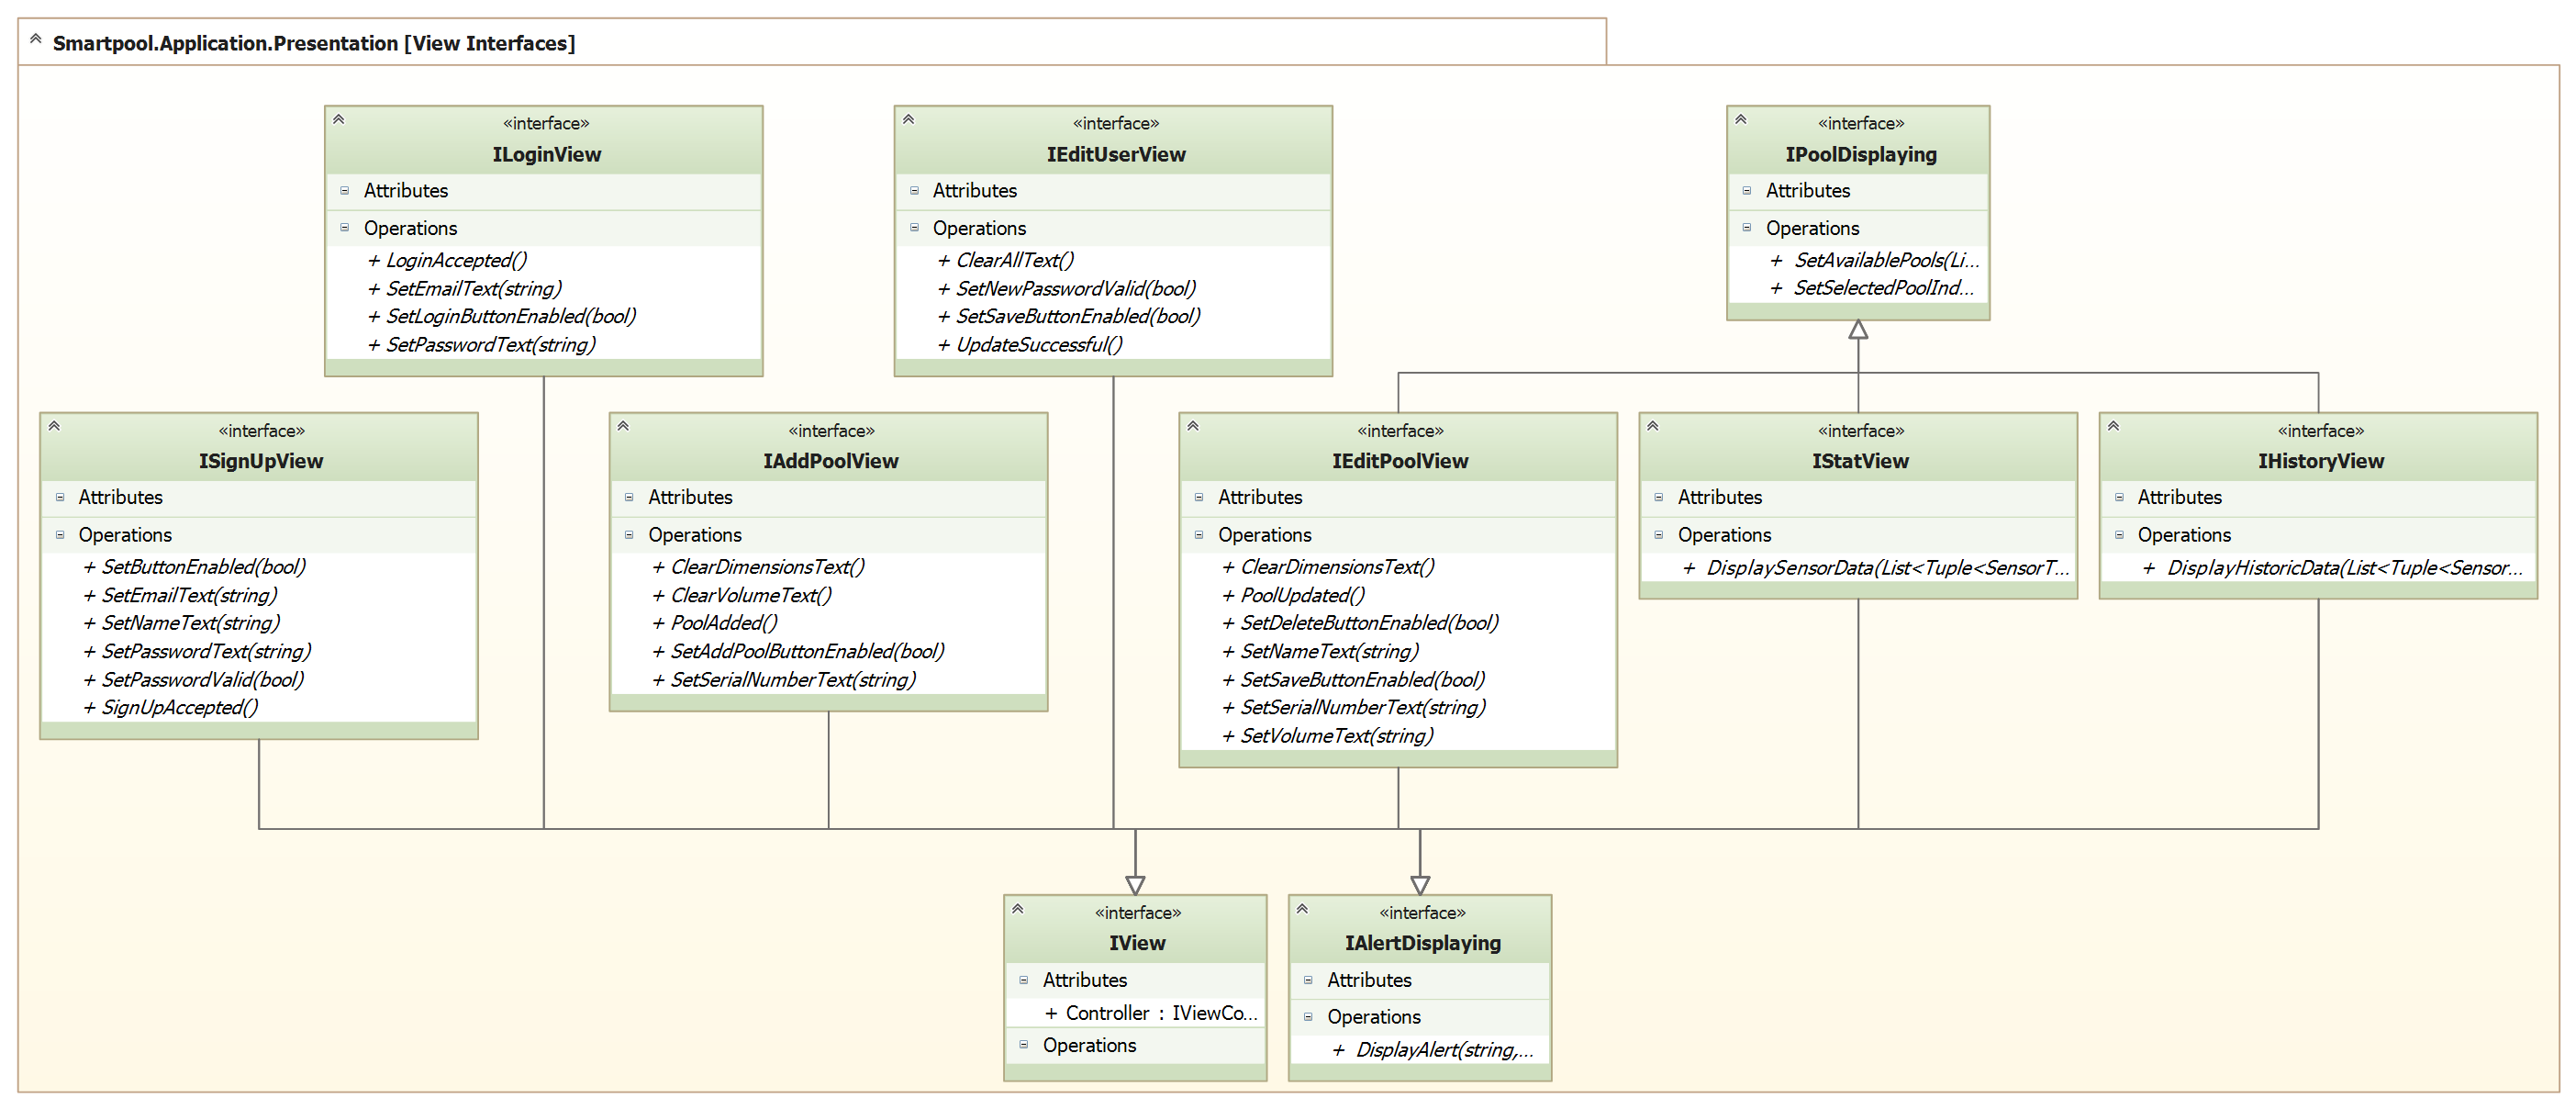
\includegraphics[width=1.0\linewidth]{figs/design/application_view_interfaces}
	\caption{View interfaces}
	\label{fig:application_view_interfaces}
\end{figure}

I de efterfølgende afsnit beskrives designet af applikationslagets view-interfaces.

\subsubsection{IView}
Dette interface er det mest generelle view-interface, som implementeres af alle de andre views. Interfacet indeholder en property, Controller, som er en IViewController beskrevet i foregående afsnit. Alle views har derfor en controller, som de kan kalde ViewDidLoad på, eller typecaste til en mere specifik controller, som passer til det konkrete view.

\begin{figure}
	\centering
	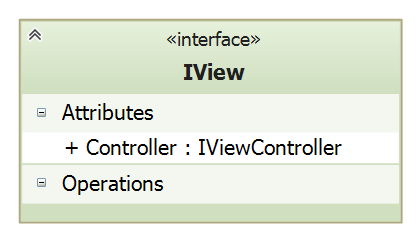
\includegraphics[width=0.3\linewidth]{figs/design/application_iview}
	\caption{IView}
	\label{fig:application_iview}
\end{figure}

\subsubsection{IPoolDisplaying}
IPoolDisplaying er et andet generelt interface, som implementeres af alle de andre view-interfaces der har med visning af pool-oplysninger at gøre. Dette interface er segregeret fra de øvrige view-interfaces i forbindelse med projektets udvikling, da flere user stories, og dermed view-designs, indeholdte metoder til visning af pool-oplysninger. Interfacet indeholder metoder, som presenteren kan kalde, for at indlæse pool-oplysninger i view?et.

\begin{figure}
	\centering
	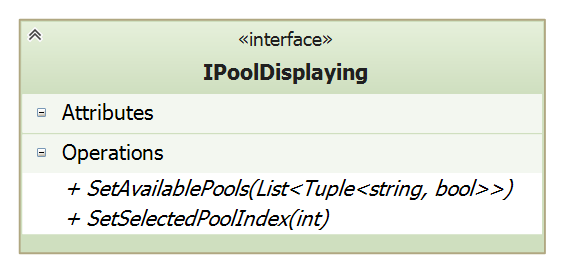
\includegraphics[width=0.4\linewidth]{figs/design/application_ipooldisplaying}
	\caption{IPoolDisplaying}
	\label{fig:application_ipooldisplaying}
\end{figure}

\subsubsection{IAlertDisplaying}
IAlertDisplaying er det sidste generelle view-interface der er designet i dette lag. Det implementeres af alle de mere specifikke view-interfaces, der bør have mulighed for at vise en notifikation for brugeren.

\begin{figure}
	\centering
	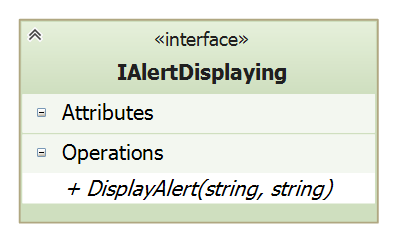
\includegraphics[width=0.3\linewidth]{figs/design/application_ialertdisplaying}
	\caption{IAlertDisplaying}
	\label{fig:application_ialertdisplaying}
\end{figure}

\subsubsection{ISignUpView}
Dette interface er modparten til ISignUpViewController interfacet. ISignUpView indeholder dermed metoder til at opdatere view?ets tilstand, i form af tekstfelter og statusnotifikationer.

\begin{table}
	\centering
	\begin{tabular}{| l | p{0.7\linewidth} |}
		\toprule
		\textbf{Klassemedlem}	& \textbf{Beskrivelse} \\
		\midrule
		+ SetButtonEnabled(...)				& En metode der ændre på hvorvidt brugeren har mulighed for at gennemføre brugeroprettelse.	\\\hline
		+ SetEmailText(...)				& Metoder til at sætte teksten i view?ets tekstfelter. \\
		+ SetNameText(...)				& \\
		+ SetPasswordText(...)				& \\\hline
		+ SetPasswordValid(...) 					& En metode der notificerer view?et, om hvorvidt de indtastede passwords kan godkendes af systemet. \\\hline
		+ SignUpAccepted()				& En metode der notificerer view?et, om at brugeroprettelsen er gennemført af systemet. \\
		\bottomrule
		\end{tabular}
	\caption{Beskrivelse af ISignUpView-klassens medlemmer}
	\label{tab:table_design_isignupview}	
\end{table}

\subsubsection{ILoginView}
ILoginView er modparten til ILoginViewController interfacet. Dette interface indeholder metoder som presenteren kan kalde, for at opdatere view?et under loginforsøg. Dette interface omhandler dermed, den user story, hvor en bruger ønsker at kunne logge ind i systemet.

\begin{table}
	\centering
	\begin{tabular}{| l | p{0.63\linewidth} |}
		\toprule
		\textbf{Klassemedlem}	& \textbf{Beskrivelse} \\
		\midrule
		+ LoginAccepted()				& En metode der notificerer view?et, når et login er gennemført.
	\\\hline
		+ SetEmailText(...)				& Metoder der sætter teksten i view?ets tekstfelter. \\
		+ SetPasswordText(...)				& \\\hline
		+ SetLoginButtonEnabled(...) 					& En metode der ændre på hvorvidt brugeren har mulighed for at gennemføre logge ind. \\
		\bottomrule
		\end{tabular}
	\caption{Beskrivelse af ILoginView-klassens medlemmer}
	\label{tab:table_design_iloginview}	
\end{table}

\subsubsection{IAddPoolView}
Dette interface er modparten til IAddPoolViewController. Det indeholder metoder der tilgodeser de user stories, hvor en pool ønskes oprettet i systemet.

\begin{table}
	\centering
	\begin{tabular}{| l | p{0.6\linewidth} |}
		\toprule
		\textbf{Klassemedlem}	& \textbf{Beskrivelse} \\
		\midrule
		+ ClearDimensionsText()				& Metoder til at slette alt tekst i de pågældende tekstfelter. \\
		+ ClearVolumeText()					& \\\hline
		+ PoolAdded()				& En metode der kaldes af presenteren, når en pool er blevet tilføjet i systemet. \\\hline
		+ SetAddPoolButtonEnabled(...)				& En metode der ændre på hvorvidt brugeren har mulighed for at tilføje en pool. \\\hline
		+ SetSerialNumberText(...) 					& En metoder der sætter teksten i view?ets serienummer tekstfelt. \\
		\bottomrule
		\end{tabular}
	\caption{Beskrivelse af IAddPoolView-klassens medlemmer}
	\label{tab:table_design_iaddpoolview}	
\end{table}

\subsubsection{IEditUserView}
IEditUserView interfacet indeholder metoder der kan kaldes af en IEditUserViewController, under redigering af pool-oplysninger.

\begin{table}
	\centering
	\begin{tabular}{| l | p{0.65\linewidth} |}
		\toprule
		\textbf{Klassemedlem}	& \textbf{Beskrivelse} \\
		\midrule
		+ ClearAllText()				& En metode der sletter alt tekst i view?ets tekstfelter. \\\hline
		+ SetPasswordValid(...)					& En metode der kan kaldes af presenteren, for at notificere view?et om hvorvidt de indtastede passwords kan godkendes.  \\\hline
		+ SetSaveButtonEnabled(...)				& En metode der ændre på hvorvidt brugeren har mulighed for at gemme ændringer om en pool.  \\\hline
		+ UpdateSuccessful()				& En metode der kaldes når en pool opdatering er gennemført af systemet. \\
		\bottomrule
		\end{tabular}
	\caption{Beskrivelse af IEditUserView-klassens medlemmer}
	\label{tab:table_design_iedituserview}	
\end{table}

\subsubsection{IEditPoolView}
Dette interface er modparten til IEditPoolViewController, og omhandler dermed redigering af pool-oplysninger. Interfacet indeholder en række metoder til at sætte tilstanden i de tekstfelter og knapper der vurderes nødvendige i views af denne type.

\begin{table}
	\centering
	\begin{tabular}{| l | p{0.62\linewidth} |}
		\toprule
		\textbf{Klassemedlem}	& \textbf{Beskrivelse} \\
		\midrule
		+ ClearDimensionsText()				 &En metode der sletter alt tekst om poolens størrelse. \\\hline
		+ PoolUpdated()					& En metode der kaldes når en pool er blevet opdateret i systemet. \\\hline
		+ SetDeleteButtonEnabled(...)				& Metoder der kaldes, for at ændre på tilstanden af knapperne i view?et. \\
		+ SetSaveButtonEnabled(...)				& \\\hline
		+ SetNameText(...)						& Metoder der kaldes, for at sætte teksten i view?ets tekstfelter.
 \\
		+ SetSerialNumberText(...)				& \\
		+ SetVolumeText(...)						& \\
		\bottomrule
		\end{tabular}
	\caption{Beskrivelse af IEditPoolView-klassens medlemmer}
	\label{tab:table_design_ieditPoolview}	
\end{table}

\subsubsection{IStatView}
IStatView er modparten til IStatViewController. Dette interface indeholder en metode, der skal kunne indlæse sensor data i view?et. Sensor data bliver sendt som en liste af tupler, med sensor type og måleværdi.

\begin{figure}
	\centering
	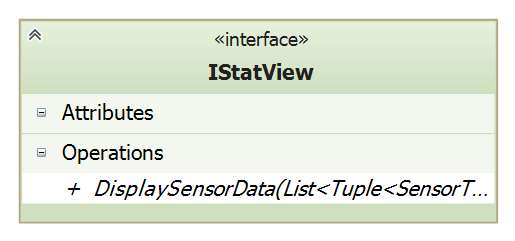
\includegraphics[width=0.3\linewidth]{figs/design/application_istatview}
	\caption{IStatView}
	\label{fig:application_istatview}
\end{figure}

\subsubsection{IHistoryView}
Dette interface er modparten til IHistoryViewController. Interface indeholder en metode, der skal kunne indlæse historisk sensor data i view?et. Sensor data bliver sendt som en liste af tupler, med sensor type og en liste af måleværdier.

\begin{figure}
	\centering
	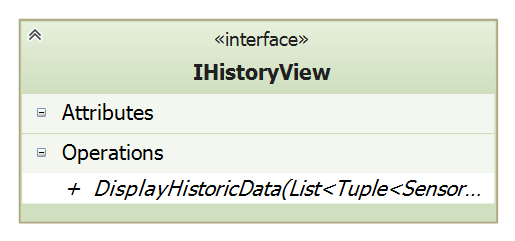
\includegraphics[width=0.3\linewidth]{figs/design/application_ihistoryview}
	\caption{IHistoryView}
	\label{fig:application_ihistoryview}
\end{figure}

\subsection{Presenter-klasser}
Efter at have designet par af view- og presenter-interfaces, blev konkrete presenter-klasser designet. De implementerer et presenter-interface, samt indeholder det view-inteface, som presenteren bør kobles sammen med.

Presenter-klasserne er designet til at være platform-uafhængige, ved ikke at benytte klasser, som ikke understøttes i portable projekter. Da klasserne er designet sammen med interfaces, giver det stadigvæk mulighed for, at lave specifikke presenters for en given platform, hvis det bliver nødvendigt. Alle presenters har en constructor, der tager imod en IClientMessenger (defineret i connection-modellen), og et view af den tilhørende type. Presenter-klasserne har brug for at modtage en IClientMessenger fra view?et der instantiere presenteren, for at platform specifikke klienter ikke skal forhindre præsentationslaget i at være portabelt. 

\begin{figure}
	\centering
	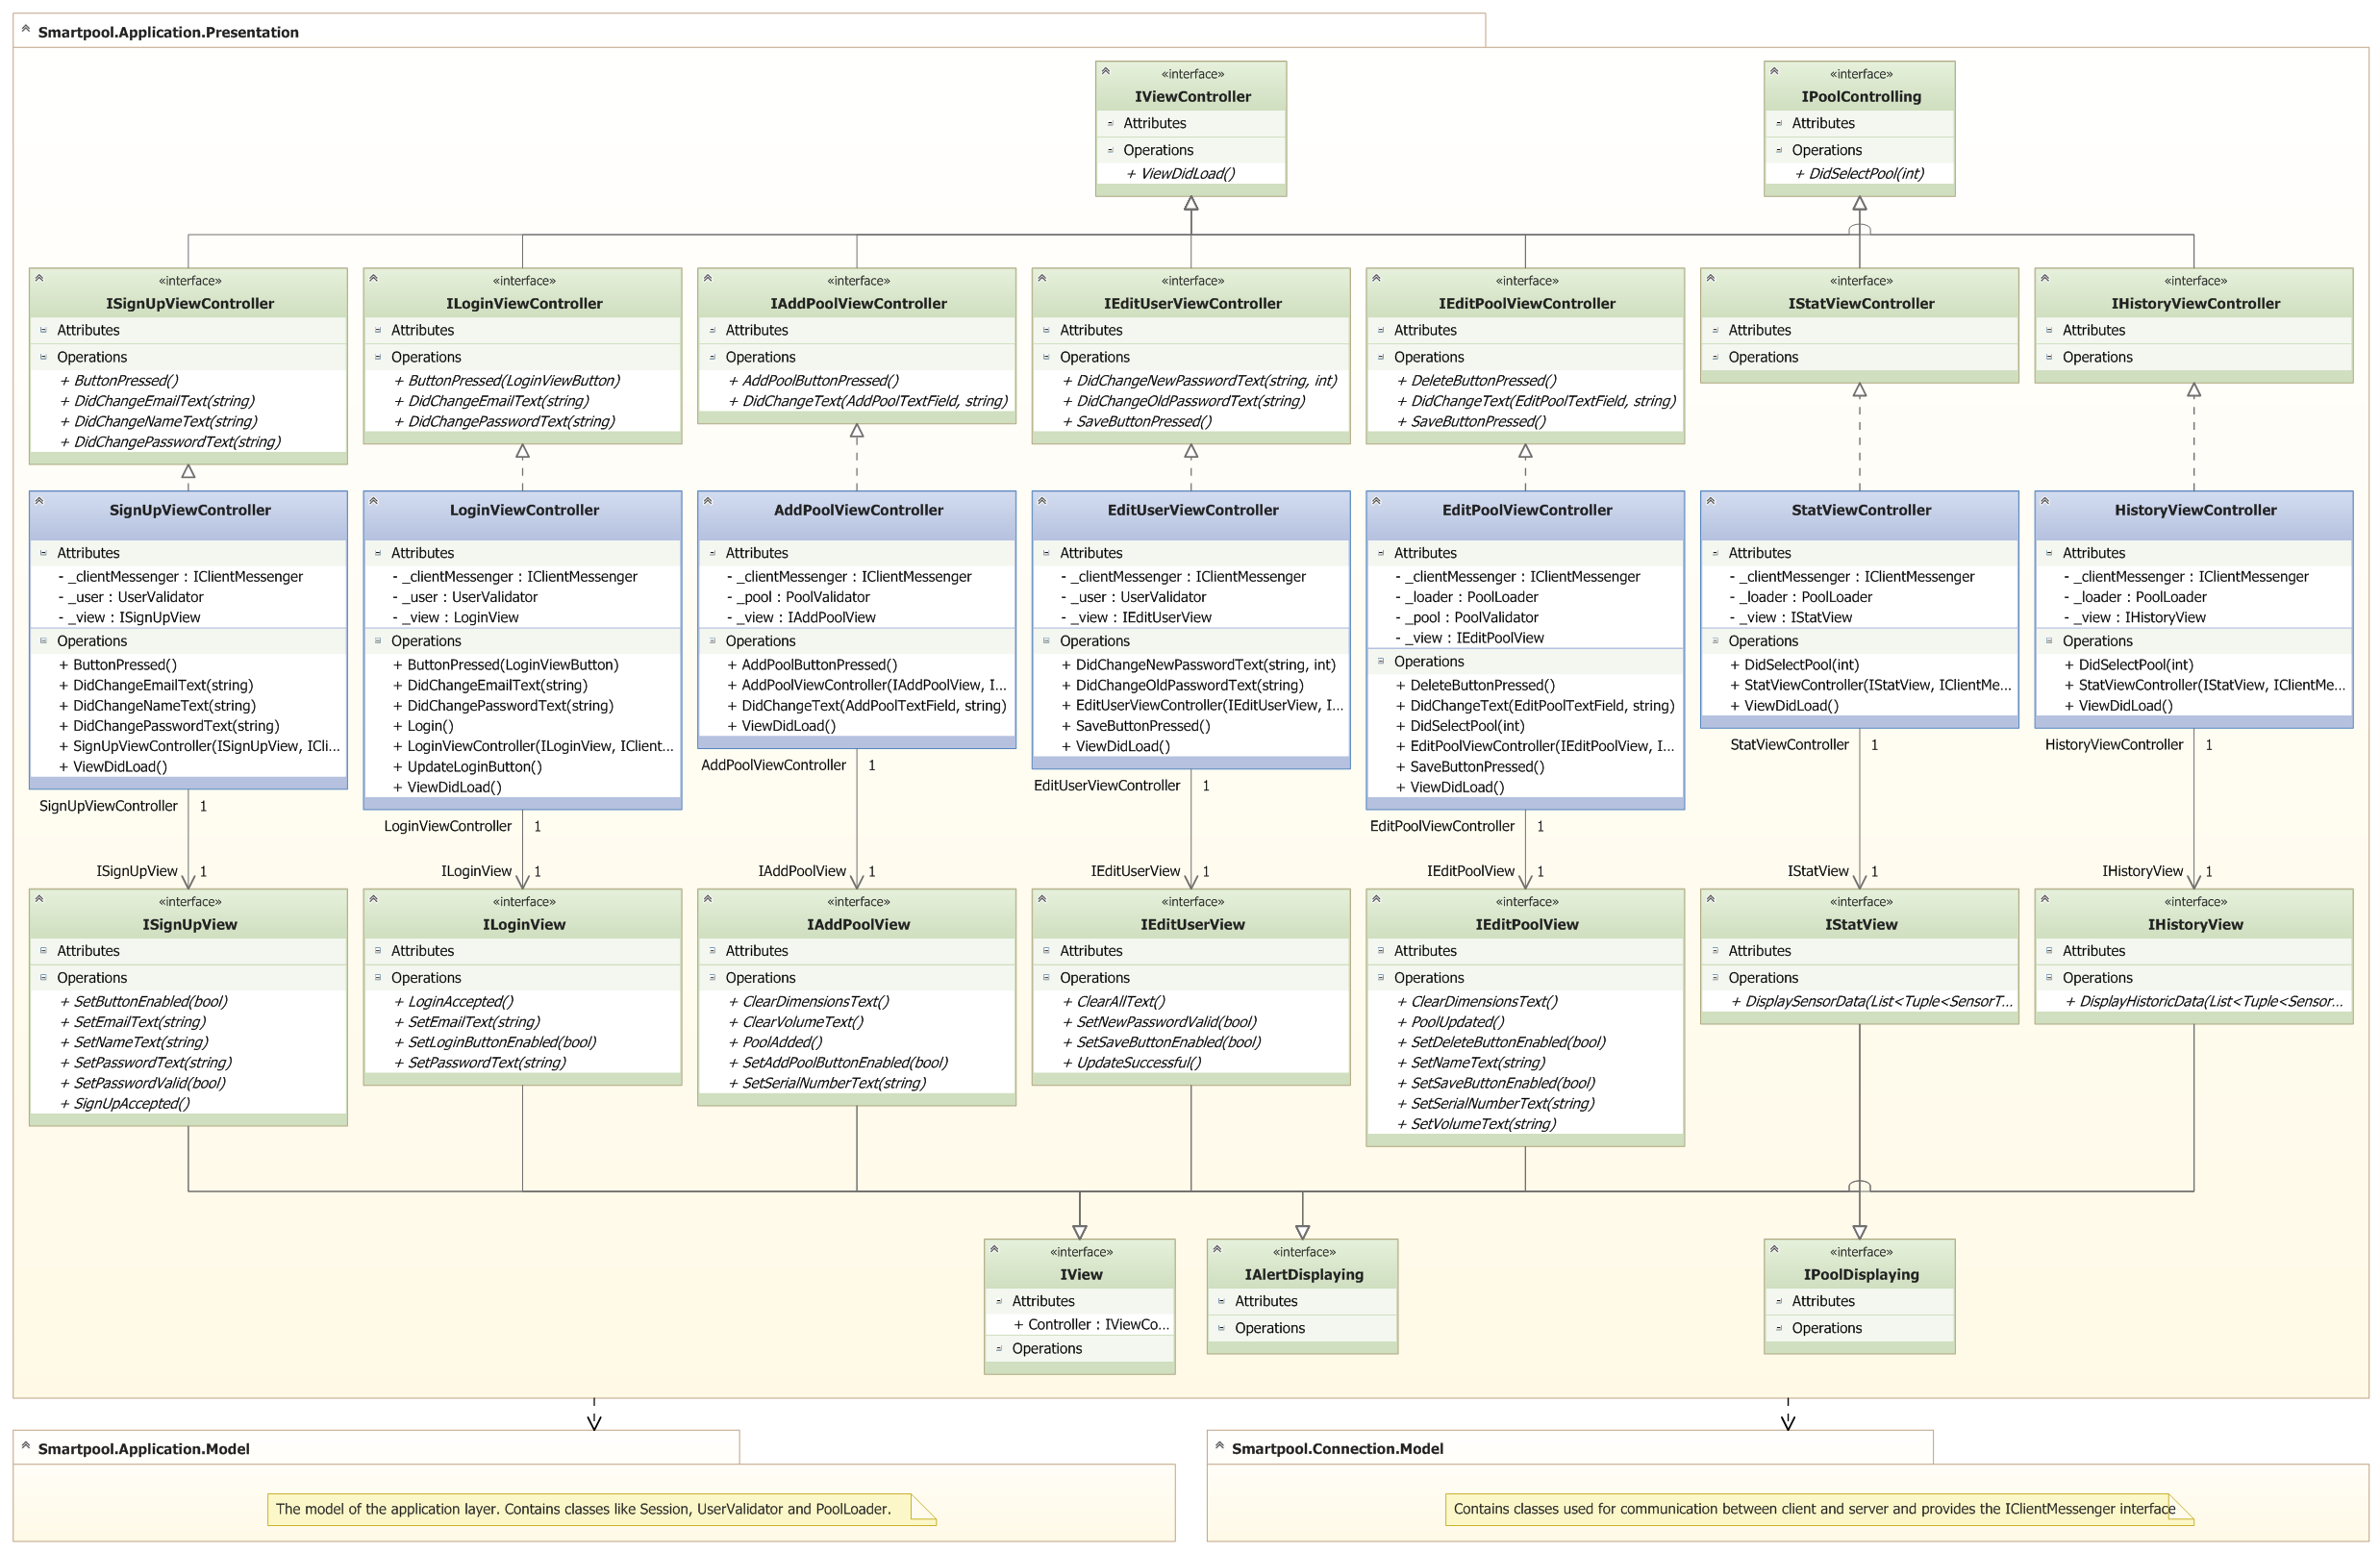
\includegraphics[width=0.9\linewidth]{figs/design/application_presentation_full}
	\caption{Klasser og interfaces i præsentationslaget}
	\label{fig:application_presentation_full}
\end{figure}\todo{skal muligvis i en pdf for sig, readability you know...}

I de efterfølgende afsnit beskrives kort, de metoder og properties, der er tilføjet designet af de konkrete presenters, og som ikke er beskrevet ved deres interface.

\subsubsection{SignUpViewController}
SignUpViewController-klassen implementerer ISignUpViewController interfacet. Klassen indeholder en række private felter, til at gemme en reference til de parametre der medsendes i constructoren. Derudover indeholder klassen en UserValidator fra modellaget, da denne type presenter har brug for en metode til, at verificere oplysninger ved brugeroprettelse.

\begin{figure}
	\centering
	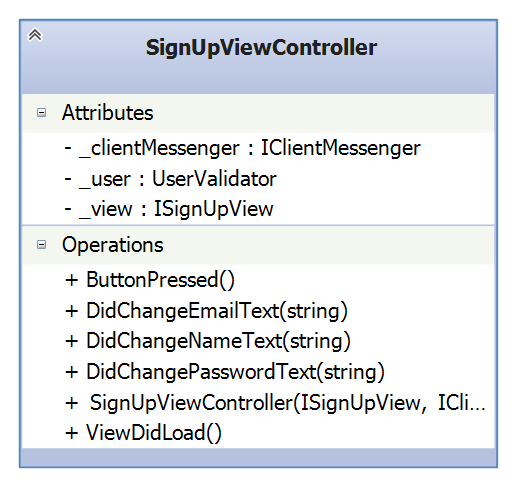
\includegraphics[width=0.3\linewidth]{figs/design/application_signupviewcontroller}
	\caption{SignUpViewController}
	\label{fig:application_signupviewcontroller}
\end{figure}

\subsubsection{LoginViewController}
LoginViewController-klassen implementerer ILoginViewController interfacet. Klassen indeholder en række private felter, til at gemme en reference til de parametre der medsendes i constructoren. Derudover indeholder klassen en UserValidator, som presenteren kan benytte til verificering af loginoplysninger.

\begin{figure}
	\centering
	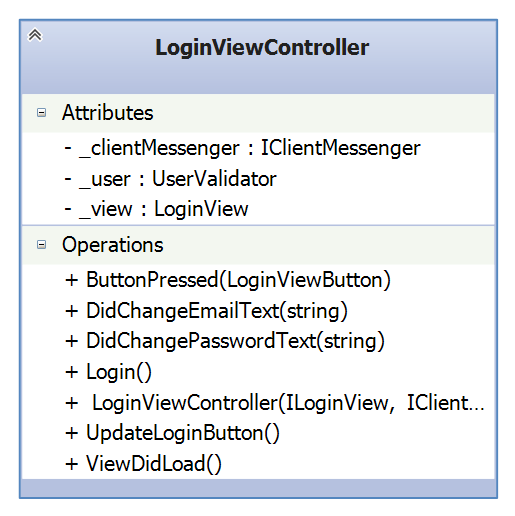
\includegraphics[width=0.3\linewidth]{figs/design/application_loginviewcontroller}
	\caption{LoginViewController}
	\label{fig:application_loginviewcontroller}
\end{figure}

\subsubsection{AddPoolViewController}
AddPoolViewController-klassen implementerer IAddPoolViewController interfacet. Klassen indeholder en række private felter, til at gemme en reference til de parametre der medsendes i constructoren. Da denne type presenter ifølge interfacet håndterer tilføjelse af nye pools, indeholder klassen også en PoolValidator fra modellaget, til validering af brugerens input.

\begin{figure}
	\centering
	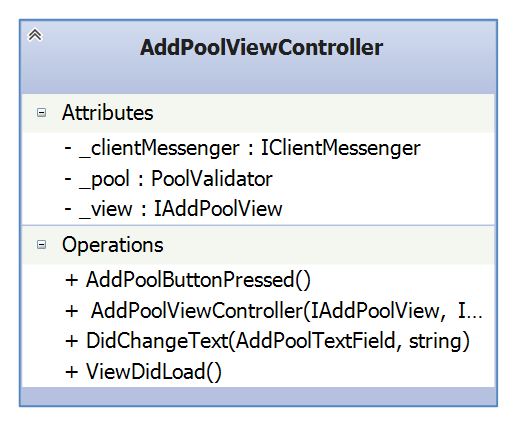
\includegraphics[width=0.3\linewidth]{figs/design/application_addpoolviewcontroller}
	\caption{AddPoolViewController}
	\label{fig:application_addpoolviewcontroller}
\end{figure}

\subsubsection{EditUserViewController}
EditUserViewController-klassen implementerer IEditUserViewController interfacet. Klassen indeholder en række private felter, til at gemme en reference til de parametre der medsendes i constructoren. Klassen har også en UserValidator til verificeing af brugeroplysninger.

\begin{figure}
	\centering
	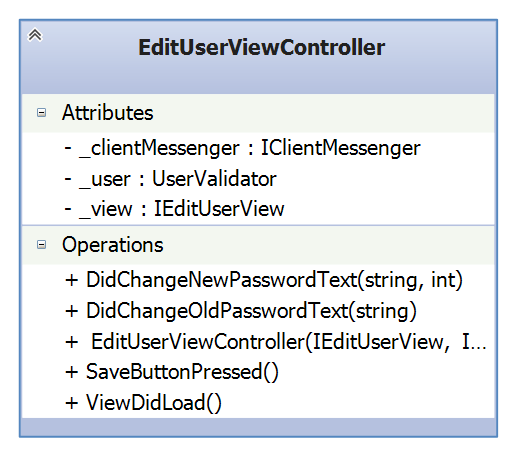
\includegraphics[width=0.3\linewidth]{figs/design/application_edituserviewcontroller}
	\caption{EditUserViewController}
	\label{fig:application_edituserviewcontroller}
\end{figure}

\subsubsection{EditPoolViewController}
Denne klasse implementerer IEditPoolViewController interfacet. Ud over de parametre der medsendes i constructoren, indeholder klassen en PoolValidator fra modellaget, samt en PoolLoader. PoolLoaderen er nødvendig for presenterens design, da den skal løse opgaver omhandlende indhentning af pool-oplysninger.

\begin{figure}
	\centering
	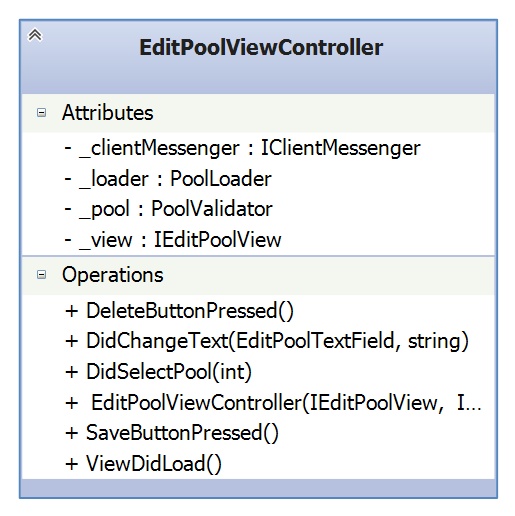
\includegraphics[width=0.3\linewidth]{figs/design/application_editpoolviewcontroller}
	\caption{EditPoolViewController}
	\label{fig:application_editpoolviewcontroller}
\end{figure}

\subsubsection{StatViewController og HistoryViewController}
StatViewController og HistoryViewController implementerer hhv. IStatViewController og IHistoryViewController interfacene. Begge presenter-klasser indeholder private felter til at gemme de parametre der modtages i constructoren, samt en PoolLoader, da begge klasser skal kunne indlæse pool-oplysninger.

\begin{figure}
	\centering
	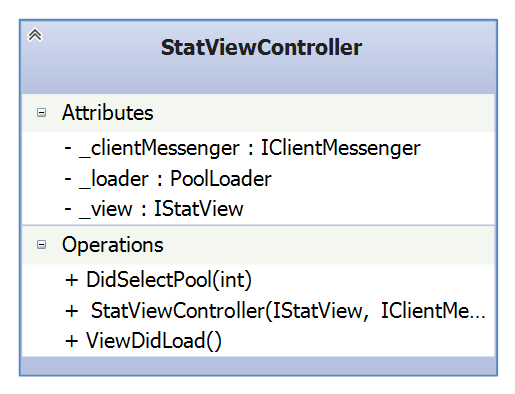
\includegraphics[width=0.3\linewidth]{figs/design/application_statviewcontroller}
	\caption{StatViewController}
	\label{fig:application_statviewcontroller}
\end{figure}